\chapter{假设检验}
\begin{example}{零件检测}{component test}
	一大批电子元件寿命$X$,样本$X_1,\ldots,X_n$
	\begin{compactenum}
		\item 若假设$X\sim\Expo(\lambda)$,那么$\lambda=\,?$

		回答:参数估计
		\item 若合格标准为$\E(X)\geqslant 5000$,那么如何判断这一批是否合格?
		
		尝试回答:建立执行标准,比如样本$\avg X>\ell$,那么$\ell=\,?$

		%样本多大程度上支持假设?
	\end{compactenum}
\end{example}
参数估计是对参数一无所知;假设检验是对参数有所了解,但有怀疑猜测需要证实。
\section{基本概念}
\begin{definition}{统计假设}{hypothesis}
	假设(hypothesis)是对一个或多个总体的某种推断或猜测。
	\begin{compactitem}
		\item 原假设(null hypothesis) $H_0$:被检验的假设;
		\item 备择假设(alternative \textasciitilde) $H_1$:拒绝$H_0$后可供选择的假设。
	\end{compactitem}
	简单假设:只对应一个总体;复合假设:对应多个总体
\end{definition}
若假设可表示为参数形式,则
\[
	H_0:\theta\in\varTheta_0,\quad H_1:\theta\in\varTheta_1
\]
其中$\varTheta_0\cap\varTheta_1=\varnothing,\enspace\varTheta_0\cup\varTheta_1=\{\theta\,\text{的所有可能取值(应用角度)\}}$。
\begin{example}{}{}
	接\exmref{exm:component test},
	\[
		H_0:\mu\geqslant\mu_0,\quad H_1:\mu<\mu_0,
	\]
	$H_0$是复合假设,单侧检验(看$H_1$)。
	\tcblower
	$X\sim\Norm(\mu,\sigma_0^2)$,
	\[
		H_0:\mu=\mu_0,\quad H_1:\mu\neq\mu_0,
	\]
	$H_0$是简单假设($\sigma_0^2$已知的情况下),双侧检验(看$H_1$)。
\end{example}

$H_0$往往是受保护的,无充分证据不能拒绝;$H_1$往往是真正感兴趣的。
\begin{theorem}{小概率原理}{}
	在假设$H_0$为真的情况下,所观测的样本出现的概率如果很小,意味着样本提供的证据拒绝$H_0$。
	%概率很小的事件在一次试验中是不会发生的;在一次试验中小概率事件如果发生了,我们就有理由认为提出的$H_0$是不对的。
\end{theorem}
%小概率由研究者事先确定,一般取1\%, 5\%或10\%。小概率的取值不同,假设检验的结果可能不同。
在统计学中,小概率又叫\textbf{显著性水平},因此,假设检验又称为\textbf{显著性检验}。一般来说,我们都希望拒绝$H_0$得到所谓的显著性差异。
\begin{definition}{假设检验}{hypothesis test}
	检验(准则):做出决策的一个具体法则。

	$R$:临界域(或拒绝域,critical region),形式上可抽象为
	\[
		R=\set{(X_1,\ldots,X_n)}{T(X_1,\ldots,X_n)\geqslant c}.
	\]
	$c$称为临界值。
\end{definition}

\begin{definition}{两类错误}{}
	\begin{compactenum}[I]
		\item 弃真错误:$H_0$为真时拒绝$H_0$,概率 
		\begin{equation}
			\alpha(R):=\P_\theta\bigkh{(X_1,\ldots,X_n)\in R},\quad \theta\in\varTheta_0
		\end{equation}
		\item 取伪错误:$H_0$为假时接受$H_0$,概率
		\begin{equation}
			\beta(R):=\P_\theta\bigkh{(X_1,\ldots,X_n)\notin R},\quad \theta\in\varTheta_1
		\end{equation}
	\end{compactenum}
\end{definition}
依据样本决策,错误不可避免。当$n$固定时,$\alpha,\beta$不能同时变小。
\begin{center}
	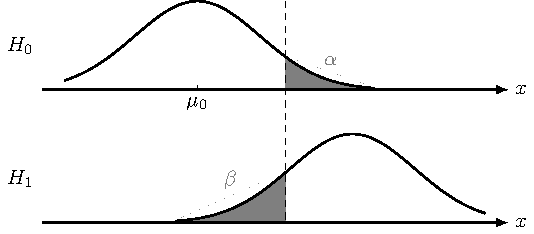
\includegraphics{figures/tikz/type-error.pdf}
	\captionof{figure}{I类错误和II类错误示意图}
\end{center}
\begin{definition}{功效函数}{power function}
	定义功效函数(power function)是样本落在$R$上的概率
	\begin{equation}
		\P_\theta\bigkh{(X_1,\ldots,X_n)\in R}=\begin{cases}
			\alpha(R),&\theta\in\varTheta_0\\
			1-\beta(R),&\theta\in\varTheta_1
		\end{cases}
	\end{equation}
	功效指在$H_1$成立时拒绝$H_0$的概率,即$1-\beta(R)$,越大越好。
\end{definition}
\begin{theorem}{Neyman-Pearson范式}{Neyman-Pearson normal form}
	($n$固定)预先给定检验水平$\alpha>0$,控制
	\[
		\alpha(R)\leqslant\alpha,\enspace\forall\theta\in\varTheta_0,
	\]
	再在这个限制下使$\beta(R)$尽可能小。
\end{theorem}
$\alpha$固定时,使$\beta(R)$最小的检验称为水平$\alpha$下的\textbf{一致最优检验}(不一定存在,即使存在一般也不易求)


\section{临界值检验法}
\begin{method}{临界值检验法}{}
	\begin{compactenum}
		\item 提出假设$H_0,H_1$
		\item 给定$\alpha>0$
		\item 选择检验统计量,确定拒绝域形状(由$H_1$决定)
		\item 构建检验:$\alpha(R)\leqslant\alpha\rightsquigarrow R$
		\item 采样,计算检验统计量的值
		\item 代入检验准则,进行决策
	\end{compactenum}
\end{method}
这个过程缺少对于功效$1-\beta(R)$的讨论。
\begin{example}{$Z$检验法和$t$检验法}{Z test & t test}
	$X\sim\Norm(\mu,\sigma^2)$,$\sigma^2$已知, 
	\[
		H_0:\mu=\mu_0,\quad H_1:\mu\neq\mu_0,
	\]
	当$H_0$为真时,由式\eqref{sample-N},选择统计量
	\[
		Z:=\frac{\avg X-\mu_0}{\sigma/\sqrt n}\sim\Norm(0,1),
	\]
	显著性水平$\alpha>0$给定,检验的拒绝域为
	\[
		C=\set{Z}{\abs Z\geqslant z_{\alpha/2}}.
	\]
	这被称为$Z$检验法。
	\tcblower
	当$\sigma^2$未知时,就需要选择统计量
	\[
		t:=\frac{\avg X-\mu_0}{S/\sqrt n}\sim\mathrm t(n-1),
	\]
	相应的,检验的拒绝域为
	\[
		C=\set{Z}{\abs t\geqslant t_{\alpha/2}(n-1)}.
	\]
	这被称为$t$检验法。
\end{example}
\begin{center}
	\captionof{table}{假设检验}
	\begin{tabular}{cccc}
		\toprule
		条件&$H_0$&统计量&拒绝域\\
		\midrule
		$\sigma^2$已知&$\mu=\mu_0$&$Z:=\frac{\avg X-\mu_0}{\sigma/\sqrt n}\sim\Norm(0,1)$&$\abs Z\geqslant z_{\alpha/2}$\\[2ex]
		$\sigma^2$未知&$\mu=\mu_0$&$t:=\frac{\avg X-\mu_0}{S/\sqrt n}\sim\mathrm t(n-1)$&$\abs t\geqslant t_{\alpha/2}(n-1)$\\[2ex]
		\multirow{2}*{$\mu$未知}&\multirow{2}*{$\sigma^2=\sigma_0^2$}&\multirow{2}*{$\chi^2:=\frac{(n-1)S^2}{\sigma_0^2}\sim\chi^2(n-1)$}&$\chi^2\geqslant\chi^2_{\alpha/2}(n-1)$或\\
		&&&$\chi^2\leqslant\chi^2_{1-\alpha/2}(n-1)$\\
		\bottomrule
	\end{tabular}
\end{center}
当$H_0$形如$\mu\geqslant\mu_0$时,进行单侧检验。
\paragraph{Review}
\begin{compactenum}
	\item $H_0$ v.s. $H_1$,二者天然不对等
	
	若认可某一组样本,则用它来证实或证伪某理论(推测);
	\item 决策:拒绝$H_0$或不拒绝$H_0$
	
	检验(准则) =决策准则,拒绝域$R$的划分
	\item 统计学中没有绝对的证实或证伪,
	
	$\alpha,\beta$属于检验程序的属性,而非样本的属性。
	
	$\alpha(R)\leqslant\alpha,\beta(R)\leqslant\beta$预先指定的可接受的长期错误率。
	\item 功效函数v.s.功效,
	
	不拒绝v.s.接受:$\beta(R)$小(功效大),当样本支持$H_0$,才能接受$H_0$;通常人们忽略了对II类错误的系统控制,将导致对结果意义以及下一步工作方向的误判。
	\item 临界值检验法。缺少对功效的讨论
\end{compactenum}
\section{临界值检验与置信区间的对偶关系}
\begin{example}{正态分布的临界值检验与置信区间}{}
	$X\sim\Norm(\mu,\sigma^2)$,$\sigma^2$已知,$\alpha\in(0,1)$给定,$X_1,\ldots,X_n$ iid 

	(双侧)置信区间
	\[
		\mu\in\kh{\avg X\pm z_{\alpha/2}\frac\sigma{\sqrt n}}.
	\]
	假设检验:考虑
	\[
		H_0:\mu=\mu_0,\quad H_1:\mu\neq\mu_0.
	\]
	%由
	%\P_{\mu=\mu_0}\Bigkh{\abs{\avg X-\mu_0}\geqslant c}\leqslant\alpha
	检验:%当$\abs{\avg X-\mu_0}\geqslant z_{\alpha/2}\sigma/\sqrt n$时拒绝$H_0$,
	接受域
	\[
		R\c=\set{(X_1,\ldots,X_n)}{\abs{\avg X-\mu_0}<z_{\alpha/2}\frac\sigma{\sqrt n}}.
	\]
\end{example}
\begin{theorem}{临界值检验与置信区间的对偶关系}{}
	\begin{center}
		置信区间包含$\mu_0$\\
		$\Updownarrow$\\
		用$\avg X$做检验统计量,建设检验$H_0:\mu=\mu_0\enspace H_1:\mu\neq\mu_0$不拒绝$H_0$
	\end{center}
\end{theorem}
\begin{remark}
	区间估计的信息更丰富,可作为证据强弱的体现。
\end{remark}
\section{\textit{P}值检验法}
\begin{example}{}{}
	$X\sim\Norm(\mu,\sigma^2)$,$\sigma^2=25$,考虑
	\[
		H_0:\mu=10,\quad H_1:\mu\neq  10,
	\]
	$n=100$,观测到的均值$\avg x=10.935$
	
	检验:若给定$\alpha=0.05$,则
	\[
		\abs{\avg x-10}=0.935<1.96\times\frac{5}{\sqrt{100}}\implies\text{不拒绝}~H_0;
	\]
	若给定$\alpha=0.1$,则
	\[
		\abs{\avg x-10}=0.935>1.65\times\frac{5}{\sqrt{100}}\implies\text{拒绝}~H_0.
	\]
	\[
		\P(|\avg X-10|\geqslant\abs{\avg x-10})=\P(\abs Z\geqslant 1.87)=0.0614.
	\]
	\begin{center}
		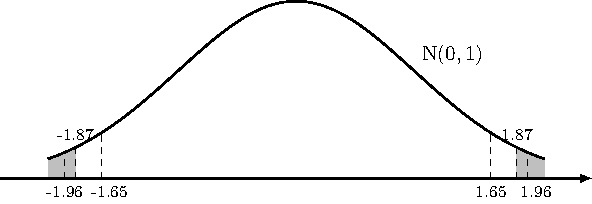
\includegraphics{figures/tikz/Pvalue.pdf}
		\captionof{figure}{$P$值检验}
		\label{fig:P value}
	\end{center}
\end{example}
\begin{definition}{检验$P$值}{}
	定义当$H_0$为真时,检验统计量的观测值以及更极端的观测出现的概率称为检验的$P$值。
\end{definition}
当$P$值$\leqslant\alpha$时拒绝$H_0$,也称为观测值显著。
\begin{compactenum}
	\item $P$值$=\P(\text{观测值及更极端的观测}|H_0)\neq\P(H_0|\text{观测值})$
	\item 若$P$值不小,则不拒绝$H_0$,原因可能为:(a) $H_0$为真;(b) $H_0$为假,但检验功效低。
\end{compactenum}
\begin{method}{$P$值检验法}{}
	\begin{compactenum}
		\item 提出假设$H_0,H_1$
		\item 给定$\alpha>0$
		\item 选择检验统计量,确定“极端”的形式(由$H_1$决定)
		\item 采样,计算检验统计量的值
		\item 计算$P$值
		\item 比较$P$值与$\alpha$,进行决策
	\end{compactenum}
\end{method}
\begin{example}{选举问题}{}
	$n=1200$,调查到的支持比例为
	\[
		\frac{684}{1200}\doteq 0.57=:p_n,
	\]
	考虑 
	\[
		H_0:p=p_0,\quad H_1:p>p_0.
	\]
	检验统计量$P_n$,由CLT
	\[
		\frac{P_n-p}{\sqrt{p(1-p)/n}}\dotsim\Norm(0,1)
	\]
	当$H_0$为真时,
	\[
		Z:=\frac{P_n-p_0}{se(P_0)}\dotsim\Norm(0,1),\quad se(P_n)=\sqrt{\frac{p_0(1-p_0)}n}.
	\]
	则$P$值
	\[
		\P_{p=p_0}(P_n\geqslant p_n)\doteq\P(Z\geqslant z_0),\quad z_0:=\frac{p_n-p_0}{se(P_n)}
	\]
	若$p_0=0.55$,则$P$值$=0.081$;若$p_0=0.5$,则$P$值$\ll 0.01$。
	\tcblower
	考虑复合假设 
	\[
		H_0:p\leqslant p_0,\quad H_1:p>p_0.
	\]
	可以取
	\[
		\hat{se}(P_n)=\sqrt{\frac{p_n(1-p_n)}n}=0.014
	\]
	当原假设为真时
	\[
		\P_{p\leqslant p_0}(P_n\geqslant p_n)\doteq\P_{p\leqslant p_0}\biggkh{Z\geqslant\frac{p_n-p}{\hat{se}(P_n)}}%\doteq 1-\Phi\biggkh{\frac{p_n-p}{\hat{se}(P_n)}},\quad p\leqslant p_0
	\]
	若拒绝$H_0:\theta\in\varTheta_0\iff T(X_1,\ldots,X_n)\geqslant c$,则
	\[
		\text{检验的}~P~\text{值}:=\sup_{\theta\in\varTheta_0}\P_{\theta}\Bigfkh{T(X_1,\ldots,X_n)\geqslant T(x_1,\ldots,x_n)}
	\]
	故
	\[
		P~\text{值}=\sup_{p\leqslant p_0}\P\biggkh{Z\geqslant\frac{p_n-p}{\hat{se}(P_n)}}=\P\biggkh{Z\geqslant\frac{p_n-p_0}{\hat{se}(P_n)}}.
	\]
	同$p=p_0$的情况。
\end{example}
\section{Bayes假设检验}
\begin{example}{}{Bayes test}
	掷10次硬币,观测到正面朝上$x$次
	\[
		H_0:p=0.5,\quad H_1:p=0.7,
	\]
	则
	\begin{equation}
		\label{eq:Bayes test}
		\frac{\P(H_0|x)}{\P(H_1|x)}=\frac{\P(H_0)\P(x|H_0)}{\P(H_1)\P(x|H_1)}<1\enspace(\text{或}\ll 1)
	\end{equation}
	时拒绝$H_0$
\end{example}
若$H_0:\theta=\theta_0$,$\varTheta$连续,则$\P(H_0|x)=\P(\varTheta=\theta_0|x)\equiv 0$,此时需要技术性处理,可参考陈5.2.8
\paragraph{Review}
\begin{compactenum}
	\item Neyman-Pearson假设检验:临界值、$P$值检验法
		Bayes假设检验,主观解释概率,引入随机变量认知参数
	\item 临界值:拒绝域形状;$P$值:更极端形式
	%\item Pearson-$\chi^2$检验是一个多项分布的检验
\end{compactenum}
\section{拟合优度检验}
\begin{theorem}{$\chi^2$检验法}{chi2 test}
	设总体$X$的分布未知,检验假设
	\begin{align*}
		H_0&:\text{总体分布函数为}~F(x)\\
		H_1&:\text{总体分布函数不是}~F(x)
	\end{align*}
	将在$H_0$下$X$可能取值的全体$\Omega$分成互不相交的子集$A_1,\ldots,A_k$,$p_i:=\P(A_i)$。
	观测到样本值$x_1,\ldots,x_n$落在$A_i$的频数为$f_i$,相应的期望频数为$np_i$,Pearson证明:
	\begin{equation}
		\chi^2:=\sum_{i=1}^k\frac{(f_i-np_i)^2}{np_i}\dotsim\chi^2(k-1).
	\end{equation}
	拒绝域$\chi^2\geqslant\chi^2_\alpha(k-1).$
\end{theorem}
推导过程见 \href{https://en.wikipedia.org/wiki/Pearson%27s_chi-squared_test}{Pearson's chi-squared test}。应用中需要$n\geqslant 50,\enspace np_i\geqslant 5$,才能较好运用这个定理。
\begin{example}{均匀的骰子}{}
	\begin{center}
		\begin{tabular}{cccccccc}
			\toprule
			点数&1&2&3&4&5&6&total\\
			\midrule
			观测频数$f_i$&4&6&17&16&8&9&60\\
			\bottomrule
		\end{tabular}
	\end{center}
	检验假设
	\[
		H_0:\text{均匀}(p_1=p_2=\cdots=p_6),\quad H_1:\text{不均匀}
	\]
	Pearson $\chi^2$统计量的观测值
	\[
		\chi^2:=\sum_{i=1}^k\frac{(f_i-np_i)^2}{np_i}=14.2.
	\]
	检验$P$值$=\P_{H_0}(\chi^2(5)\geqslant\chi^2)=0.014$
\end{example}
连续情况,划分区间,分别计算参数$\theta$的MLE $\theta^\ast$,卡方统计量分布近似$\chi^2(k-1-r)$,其中$r=\dim(\theta)$。但分别计算MLE非常麻烦。

实践中先计算$\theta$的MLE $\theta^\ast$,再划分区间,计算$p_i$,卡方统计量分布不是近似$\chi^2(k-1-r)$,但是检验$P$值介于分布$\chi^2(k-1-r)$和$\chi^2(k-1)$算得的$P$值之间。

事实:独立的卡方统计量可以合并,自由度相应的相加。
\begin{example}{Mendel豌豆试验}{}
	Mendel的试验全部独立(不同作物组),Fisher计算其每个卡方统计量并且合并,得到的卡方统计量$\chi^2=41.6056$,自由度为84,$P$值
	\[
		\P(\chi^2(84)\geqslant\chi^2)=0.99993
	\]
	\textit{were far too perfect},Fisher对这个extraordinary result没有发表任何评论,只是指出\textit{the bias seems to pervade the whole of the data.}
\end{example}
\section{列联表检验}
列联表(conttingency table)是一种按两个属性作双向分类的表。
\begin{center}
	\captionof{table}{$a\times b$列联表}
	\begin{tabular}{c|ccc|c}
		\toprule
		&A$_1$&$\cdots$&A$_a$&total\\
		\hline
		B$_1$&$n_{11}$&$\cdots$&$n_{a1}$&$n_{\cdot 1}$\\
		$\vdots$&$\vdots$&$\ddots$&$\vdots$&$\vdots$\\
		B$_b$&$n_{1b}$&$\cdots$&$n_{ab}$&$n_{\cdot b}$\\
		\hline
		total&$n_{1\cdot}$&$\cdots$&$n_{a\cdot}$&$n$\\
		\bottomrule
	\end{tabular}
\end{center}
\begin{example}{独立性检验}{independent test}
	样本写在列联表中
	\[
		H_0:~\text{独立}~(p_{ij}=p_{i\cdot}p_{\cdot j})\quad H_1:~\text{不独立}
	\]
	在$H_0$为真的前提下,估计$p_{ij}$,MLE解得
	\[
		p_{ij}^\ast=p_{i\cdot}^\ast p_{\cdot j}^\ast=\frac{n_{i\cdot}}n\frac{n_{\cdot j}}n.
	\]
	卡方统计量
	\begin{equation}
		\chi^2=\sum_{i=1}^a\sum_{j=1}^b\frac{(nn_{ij}-n_{i\cdot}n_{\cdot j})^2}{nn_{i\cdot}n_{\cdot j}}.
	\end{equation}
	自由度$=ab-1-(a-1+b-1)=(a-1)(b-1)$。
	\tcblower
	特别地,当$a=b=2$时,自由度为1
	\[
		\chi^2=\frac{n(n_{11}n_{22}-n_{12}n_{21})^2}{n_{1\cdot}n_{2\cdot}n_{\cdot 1}n_{\cdot 2}}.
	\]
\end{example}
\begin{example}{齐性检验}{}
	Jane Austen作家,仿写\footnote{A: Sense and Sensibility. B: Emma. C: Sadition (unfinished). c: Sadition (imitation)}
	\begin{center}
		\captionof{table}{Jane Austen作品单词频数}
		\begin{tabular}{c|ccc|c|c}
			\toprule
			&A&B&C&total&c\\
			\hline
			a&147&186&101&434&83\\
			an&25&26&11&62&29\\
			this&32&39&15&86&15\\
			that&94&105&37&236&22\\
			with&59&74&28&161&43\\
			without&18&10&10&38&4\\
			\hline
			total&375&440&202&1017&196\\
			\bottomrule
		\end{tabular}
	\end{center}
	(1)检验Austen不同作品中单词用法的一致性
	\[
		H_0:~\text{具有一致性}~(p_{i1}=p_{i2}=p_{i3})
	\]
	在$H_0$为真的前提下,$p_1^\ast=434/1017$等,卡方统计量观测值
	\[
		\chi^2=12.27,
	\]
	自由度为10,$P$值$\sim 0.3$,故不拒绝$H_0$。

	(2)检验仿写者与Austen不同单词的用法的一致性
	\[
		H_0:~\text{具有一致性}~(p_{i\cdot}=p_{i\mathrm c})
	\]
	可得$\chi^2=32.81$,自由度5,$P$值$<10^{-3}$,拒绝$H_0$。
\end{example}
\section{似然比检验}
\begin{example}{}{}
	接\exmref{exm:Bayes test},式\eqref{eq:Bayes test}中,考虑
	\[
		\underset{\text{后验比}}{\frac{\P(H_0|x)}{\P(H_1|x)}}=\underset{\text{先验比}}{\frac{\P(H_0)}{\P(H_1)}}\underset{\text{似然比}}{\frac{\P(x|H_0)}{\P(x|H_1)}}<1\enspace(\text{或}\ll 1)
	\]
	时拒绝$H_0$;似然比检验就是当
	\[
		\frac{\P(x|H_0)}{\P(x|H_1)}\leqslant c
	\]
	时拒绝$H_0$。
\end{example}
可以证明,当$H_0,H_1$均为简单假设时,似然比检验是最优的。

当$H_0,H_1$不是简单假设时,
\[
	H_0:\theta\in\varTheta_0\quad H_1:\theta\in\varTheta_1
\]
得到随机样本$X_1,\ldots,X_n$,定义广义似然比
\[
	\Lambda^\ast:=\frac{\sup_{\theta\in\varTheta_0}L(\theta)}{\sup_{\theta\in\varTheta_1}L(\theta)}.
\]
基于技术原因,检验统计量为
\begin{equation}
	\Lambda:=\frac{\sup_{\theta\in\varTheta_0}L(\theta)}{\sup_{\theta\in\varTheta_0\cup\varTheta_1}L(\theta)}\equiv\frac{\sup_{\theta\in\varTheta_0}L(\theta)}{L(\theta^\ast)}.
\end{equation}
易得,当$\theta^\ast\in\varTheta_0$时,$\Lambda=1>\Lambda^\ast$,当$\theta^\ast\in\varTheta_1-\varTheta_0$时,$\Lambda=\Lambda^\ast$,即
\[
	\Lambda%(X_1,\ldots,X_n)
	=\min(\Lambda^\ast,1).
\]
$\Lambda$越小则样本越不支持$H_0$。
\begin{method}{临界值检验}{}
	选择$\lambda_0$使得$\P(\Lambda\leqslant\lambda_0|H_0)\leqslant\alpha$,若$H_0$为真时$\Lambda$的分布方便求,则可直接计算$\P(\Lambda\leqslant\lambda_0|H_0)$。
\end{method}
\begin{theorem}{}{}
	在一定光滑性的条件下,%当$n\to\infty$时,
	在$H_0$为真的前提下,
	\begin{equation}
		-2\ln\Lambda\dto\chi^2(d).
	\end{equation}
	其自由度$d=\dim(\varTheta_0\cup\varTheta_1)-\dim(\varTheta_0)$,$\dim$表示自由参数的个数。
\end{theorem}
\begin{example}{多项分布的似然比估计}{}
	多项分布
	\[
		H_0:p_1=p_1^0,\ldots,p_k=p_k^0,\enspace(p_1^0+\cdots+p_k^0=1)
	\]
	观测频数$n_1,\ldots,n_k$,$n_1+\cdots+n_k=n$,似然函数
	\[
		L(p_1,\ldots,p_k)=\binom n{n_1,\ldots,n_k}p_1^{n_1}\cdots p_k^{n_k},
	\]
	故
	\[
		\Lambda=\frac{L(p_1^0,\ldots,p_k^0)}{L(p_1^\ast,\ldots,p_k^\ast)},\quad p_i^\ast=\frac{n_i}n.
	\]
	则
	\begin{align*}
		-2\ln\Lambda&=-2\sum_{i=1}^k n_i\ln\biggkh{\frac{p_i^0}{p_i^\ast}}=2\sum_{i=1}^kn_i\ln\biggkh{\frac{n_i}{np_i^0}}\\
		&=\cancel{2\sum_{i=1}^k(n_i-np_i^0)}+\sum_{i=1}^k\frac{(n_i-np_i^0)^2}{np_i^0}+\cdots
	\end{align*}
	$\dim(\varTheta_0)=0,\enspace\dim(\varTheta_0\cup\varTheta_1)=k-1$
\end{example}
\section{两总体的比较}
两独立总体$X,Y$比较,均值方差分别为$\mu_1,\mu_2,\sigma_1^2,\sigma_2^2$

\begin{example}{比较成功率}{}
	阿司匹林对于降低心脏病发病率的有效性(历时5年),样本信息:
	\begin{center}
		\captionof{table}{阿司匹林}
		\begin{tabular}{c|cccc}
			\toprule
			&心脏病发作&未发作&合计&发作率\\
			\midrule
			安慰剂&239&10795&11034&0.0217\\
			阿司匹林&129&10898&11037&0.0126\\
			\bottomrule
		\end{tabular}
	\end{center}
	安慰剂和阿司匹林组的发作率为$p_1,p_2$,假设检验 
	\[
		H_0:p_1=p_2\,(\text{无效}),\quad H_1:p_1>p_2\,(\text{有效})
	\]
	故
	\[
		\E(P_1-P_2)=p_1-p_2,\enspace\Var(P_1-P_2)=\frac{p_1(1-p_1)}{n_1}+\frac{p_2(1-p_2)}{n_2}.
	\]
	且
	\[
		\frac{(P_1-P_2)-(p_1-p_2)}{\hat{se}}\dotsim\Norm(0,1),
	\]
	在$H_0$为真的前提下,$p_1=p_2=:p$,
	\[
		p^\ast=\frac{k_1+k_2}{n_1+n_2},\enspace\hat{se}=\sqrt{p^\ast(1-p^\ast)\biggkh{\frac1{n_1}+\frac1{n_2}}}=0.00175
	\]
	检验$P$值$=\P(Z\geqslant 5.20)\ll 10^{-3}$,拒绝$H_0$。
\end{example}
\begin{remark}
	随机分组,双盲试验,$n$充分大。
\end{remark}

\section{显著性思考}
假设检验不能解释原因,不能检验试验设计,试验者需要对样本负责。

统计显著$\neq$实际显著(陈P236)